\documentclass[glossy]{beamer}
\useoutertheme{wuerzburg}
\useinnertheme[realshadow,corners=2pt,padding=2pt]{chamfered}
\usecolortheme{shark}

\usepackage{tikz}
\usepackage{float}
\usepackage{amsthm}
\usepackage{amsmath}
\newcommand<>{\hover}[1]{\uncover#2{%
 \begin{tikzpicture}[remember picture,overlay]%
 \draw[fill,opacity=0.4] (current page.south west)
 rectangle (current page.north east);
 \node at (current page.center) {#1};
 \end{tikzpicture}}
}

\title{Lecture 7 lecture note scribe}
\author{Luxi Cao, Zongyan Wang}
\institute{Univeristy of Wisconsin, Maidson}
\date{\today}

\begin{document}

\begin{frame}
\maketitle
\end{frame}

\begin{frame}
\frametitle{Section 2.9 Frechet classes and
Frechet bounds, given univariate
margins}
\begin{itemize}
\item absolutely continuous and singular multivariate
distributions, Frechet class, Frechet bounds,
concordance ordering, comonotonic copula,
countermonotonic, measure of monotone
dependence, Kendall's $\tau$, Spearman's $\rho$ or
rank correlation, Blomqvist's $\beta$, tail
dependence.
\item Kendall's tau and Spearman's rho are very popular.
\item  tail order and form of copula density at corners,
Kullback-Leibler and Jereys divergence of copula
families, semi-correlation.
\end{itemize}
\end{frame}


\begin{frame}
\frametitle{Parametric copula families
margins}
\begin{itemize}
\item  Let's start with parametric bivariate copula
families, then generalize to multivariate, or
build multivariate copula families from
combining several bivariate families. This is the way to do vine copula. The concept of vine copula started at Europe. 
\item For a 1-parameter copula family, the amount
of dependence should increase as the
parameter increases (compare bivariate
Gaussian with parameter $-1 \leq rho \leq 1$). This statement may not be right, depends on how you define your parameter. You may define the parameter as $\xi$ or $1/\xi$, the latter one has a range of $(-\infty,\infty)$.
\end{itemize}
\end{frame}

\begin{frame}
\frametitle{Parametric copula families
margins}
\begin{itemize}
\item  Correlation is not the best measure of
dependence in general; it is a measure of
linear dependence and might not reach 1 or -1
for non-Gaussian random variables with
strongest dependence. Suppose $y = (x - a)^2$, $y$ and $x$ are strongest dependence, since $y$ and $x$ depend on each other, however, consider the linear coefficient correlation, it's roughly equal to zero. 
\item For continuous variables, extreme
dependence are perfect positive dependence
(comonotonic) and perfect negative
dependence (countermonotonic). 
\end{itemize}
\hover<2>{
  \begin{minipage}{0.8\linewidth}
   \begin{block}{linear correlation coefficient might not reach 1 or -1 even with the strongest dependence}
    \begin{figure}[H]
\centering
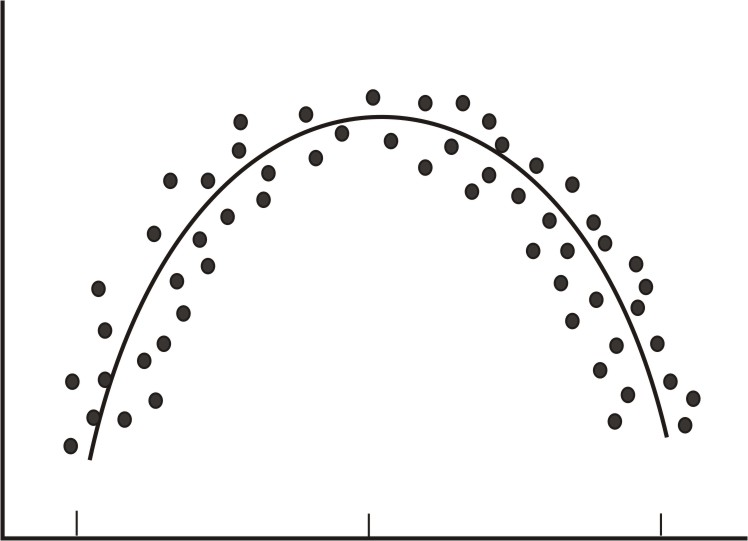
\includegraphics[width = 0.5\textwidth]{nonlinear.png}
\caption{\label{fig: non-linear correlation}May suggests $y \sim x^2$, but correlation coefficient will be approximately 0}
\end{figure}
   \end{block}
  \end{minipage}
 }

\end{frame}

\begin{frame}
\frametitle{Probability integral transform}
\begin{itemize}
\item  If $U \sim U(0,1)$, and $F$ is a univariate cdf with $F^{-1}$ (or $F^{\leftarrow}$ being the (generalized) inverse or quantile function, then $Y = F^{-1}(U) \sim F$. $Y$ can be continuous or discrete. To prove, It's easy to explain when it's continuous case, but should be careful when discrete case.
\item If $Y \sim F$ is a continuous random variable, then $F(Y) \sim U(0,1)$
\item If $F_j$ are continuous cdf for $j = 1,2$ and $Y_1 \sim F_1$, then $F_2^{-1}(F_1(Y_1)) = F_2^{-1} \cdot F_1(Y_1) \sim F_2$. (follows from above 2 items). $F_1$ and $F_2$ are determinant functions, they are not random. 
\item If $F_j$ are continuous cdfs for $j = 1,2$ and $Y_1 \sim F_1$, then $F_2^{-1}(1 - F_1(Y_1)) \sim F_2$. As long as we have uniform random variables, then $1 - U$ is still uniform distributed in (0,1).
\end{itemize}
\end{frame}

\begin{frame}
\frametitle{Absolutely continuous and singular
multivariate distributions}

\begin{itemize}
\item Special case of comonotonic: ($X_1,X_2$) such $X_1 = X_2 = U$ where $U$ is Uniform(0,1)
\item Let $X_1, X_2$ be Uniform(0,1) such that $X_1, X_2$ are equal with probability $\pi$ and independent with probability $1- \pi$. This is a mixture of singular and continuous.
\item Let $Z_1, Z_2, Z_{12}$ be independent exponential random variables with rate parameters $\eta_1, \eta_2, \eta_{12}$ respectively. Let $X_1 = min\{Z_1,Z_{12}\}$, $X_2 = min\{Z_2, Z_{12}\}$. We get singularity in joint distribution, but each of marginal is continuous. 
\end{itemize}
\end{frame}

\begin{frame}
\frametitle{$Fr\acute{e}chet$ classes, $Fr\acute{e}chet$ bounds}

\begin{itemize}
\item  $F^{-}(x_1,x_2) = max\{0, F_1(x) + F_2(x_2) - 1\} \leq F(x_1, x_2) \leq min\{F_1(x_1), F_2(x_2)\} = F^{+}(x_1,x_2) \  (2.38)$
\item \begin{align*}
Pr(A_1) + Pr(A_2) - 1 
&\leq Pr(A_1) + Pr(A_2) - Pr(A_1 \cup A_2) \\
&= Pr(A_1 \cap A_2) \\
&\leq min\{Pr(A_1), Pr(A_2)\}\\
\end{align*}
with $A_1 = \{Y_1 \leq y_1\}, A_2 = \{Y_2 \leq y_2 \}, Y_1 \sim F_1, Y_2 \sim F_2$
\item The upper bound $F^{+}$ and lower bound $F^{-}$ are distributions in $\mathcal{F}(F_1,F_2)$ for any $F_1,F_2$ whether they are discrete, continuous or mixed. 
For $F \in \mathcal{F}(F_1,..,F_d)$, $Fr\acute{e}chet$ bounds are:
$max\{0,F_1(x_1) + ... + F_d(x_d) - (d - 1)\} \leq F(x) \leq min\{F_1(x_1),... ,F_d(x_d)\} = F^{+}(x)$.
\item The upper bound $F^{+}$ is a distribution in $\mathcal{F}(F_1,... ,F_d)$ in general, but not the lower bound. It follows from $Fr\acute{e}chet$(1935) that the lower bound is point-wise sharp over $F \in \mathcal{F}(F_1, ..., F_d)$. 
\end{itemize}
\end{frame}

\begin{frame}
\frametitle{$Fr\acute{e}chet$ classes, $Fr\acute{e}chet$ bounds}

\begin{itemize}
\item  If $F_1, ..., F_d$ are continuous and $X_j \sim F_j, j = 1,..., d$, then the $Fr\mathcal{e}chet$ upper bound corresponds to comonotonic random variables with $X_j = F_j^{-1}(F_1(X_1)), j = 2,...,d,$ i.e., perfect positive dependence with $F_j^{-1} \cdot F_1$ all monotone increasing. Why? Cause all the $X_j$ are transformed by $X_1$, $j = 2, ...,d$.
\item Example 2.7 Suppose $X_1 \sim Pareto(\alpha, 1)$, and $X_2 \sim Exponential(1)$, then $X_2 = F_2^{-1}(F_1(X_1)) = -\log[(1+X_1)^{-\alpha}] = \alpha \log(1+X_1)$ is a monotone increasing functional relation but the correlation of $X_1$, $X_2$ is not 1.
\end{itemize}

 \hover<2>{
  \begin{minipage}{0.8\linewidth}
   \begin{block}{}
    \begin{proof}[Proof: Example 2.7]
$X1 = e^{X_2/\alpha} - 1, X_2 \sim Expo(1)$
\begin{align*}
Cov(X_1, X_2)
& = \int_0^{\infty} x(e^{x/\alpha} - 1) e^{-x} dx\\
& = \int_0^{\infty} x e^{-\frac{\alpha - 1}{alpha}x} - x e^{-x} dx\\
& = (\frac{\alpha - 1}{\alpha})^2 - 1 \\
& = \frac{2\alpha - 1}{(\alpha - 1)^2}
\end{align*}
Since $X_1 \sim Pareto(\alpha, 1)$, and $X_2 \sim Exponential(1)$, we have $var(X_1) = 1$, $var(X_2) = \frac{\alpha}{(\alpha - 1)^2 (\alpha - 2)}$,\\
We have $Corr(X_1, X_2) = \frac{2\alpha - 1}{(\alpha - 1)\sqrt{\alpha/(\alpha - 2)}}$
\end{proof}
   \end{block}
  \end{minipage}
 }
\end{frame}



\begin{frame}
\frametitle{$Fr\acute{e}chet$ classes, $Fr\acute{e}chet$ bounds}

\begin{itemize}
\item  If $F_1, ..., F_d$ are continuous and $X_j \sim F_j, j = 1,..., d$, then the $Fr\mathcal{e}chet$ upper bound corresponds to comonotonic random variables with $X_j = F_j^{-1}(F_1(X_1)), j = 2,...,d,$ i.e., perfect positive dependence with $F_j^{-1} \cdot F_1$ all monotone increasing. Why? Cause all the $X_j$ are transformed by $X_1$, $j = 2, ...,d$.
\item Example 2.7 Suppose $X_1 \sim Pareto(\alpha, 1)$, and $X_2 \sim Exponential(1)$, then $X_2 = F_2^{-1}(F_1(X_1)) = -\log[(1+X_1)^{-\alpha}] = \alpha \log(1+X_1)$ is a monotone increasing functional relation but the correlation of $X_1$, $X_2$ is not 1.

\item Example 2.8 Suppose $X_1$, $X_2$ are countermonotonic. If $X_1$,$X_2\sim Exp(1)$, then $X_2=F_2^{-1}(1-F_1(X_1))=F_2^{-1}(e^{-X_1})=-log[1-e^{-X_1}]$ is a monontone decreasing functional relation but the correlation of $X_1$,$X_2$ is not -1.
\end{itemize}

 \hover<2>{
  \begin{minipage}{0.9\linewidth}
   \begin{block}{}
    \begin{proof}[Proof: Example 2.8]
\begin{align*}
Corr(X_1, X_2) 
&=[E(X_1X_2)-E(X_1)E(X_2)]/\sqrt{Var(X_1)Var(X_2)} \\
&=E(X_1X_2)-1= \\
&-E(X_1log[1-e^{-X_1})-1 \\
&=-\int_0^{\infty} xlog[1-e^{-x} dx-1\\
&=0.355-1=-0.645
\end{align*}

\end{proof}
   \end{block}
  \end{minipage}
 }
\end{frame}





\begin{frame}
 \frametitle{This is a title}
 Some text
 \hover<2>{
  \begin{minipage}{0.8\linewidth}
   \begin{block}{A block hovering above the slide}
    I am visible on slide two.
   \end{block}
  \end{minipage}
 }
\end{frame}

\end{document}